\documentclass{article}

\usepackage{graphicx}
\usepackage{tikz}
\usepackage{tikzsymbols}
\usetikzlibrary{calc,patterns,shapes.geometric}
\pagestyle{empty}
\usepackage[margin=0pt]{geometry}
\geometry{papersize={14in,12in}}

\def\centerarc[#1](#2)(#3:#4:#5){\draw[#1] ($(#2)+({#5*cos(#3)},{#5*sin(#3)})$) arc (#3:#4:#5);}

\begin{document}
	\begin{figure}
		\centering
		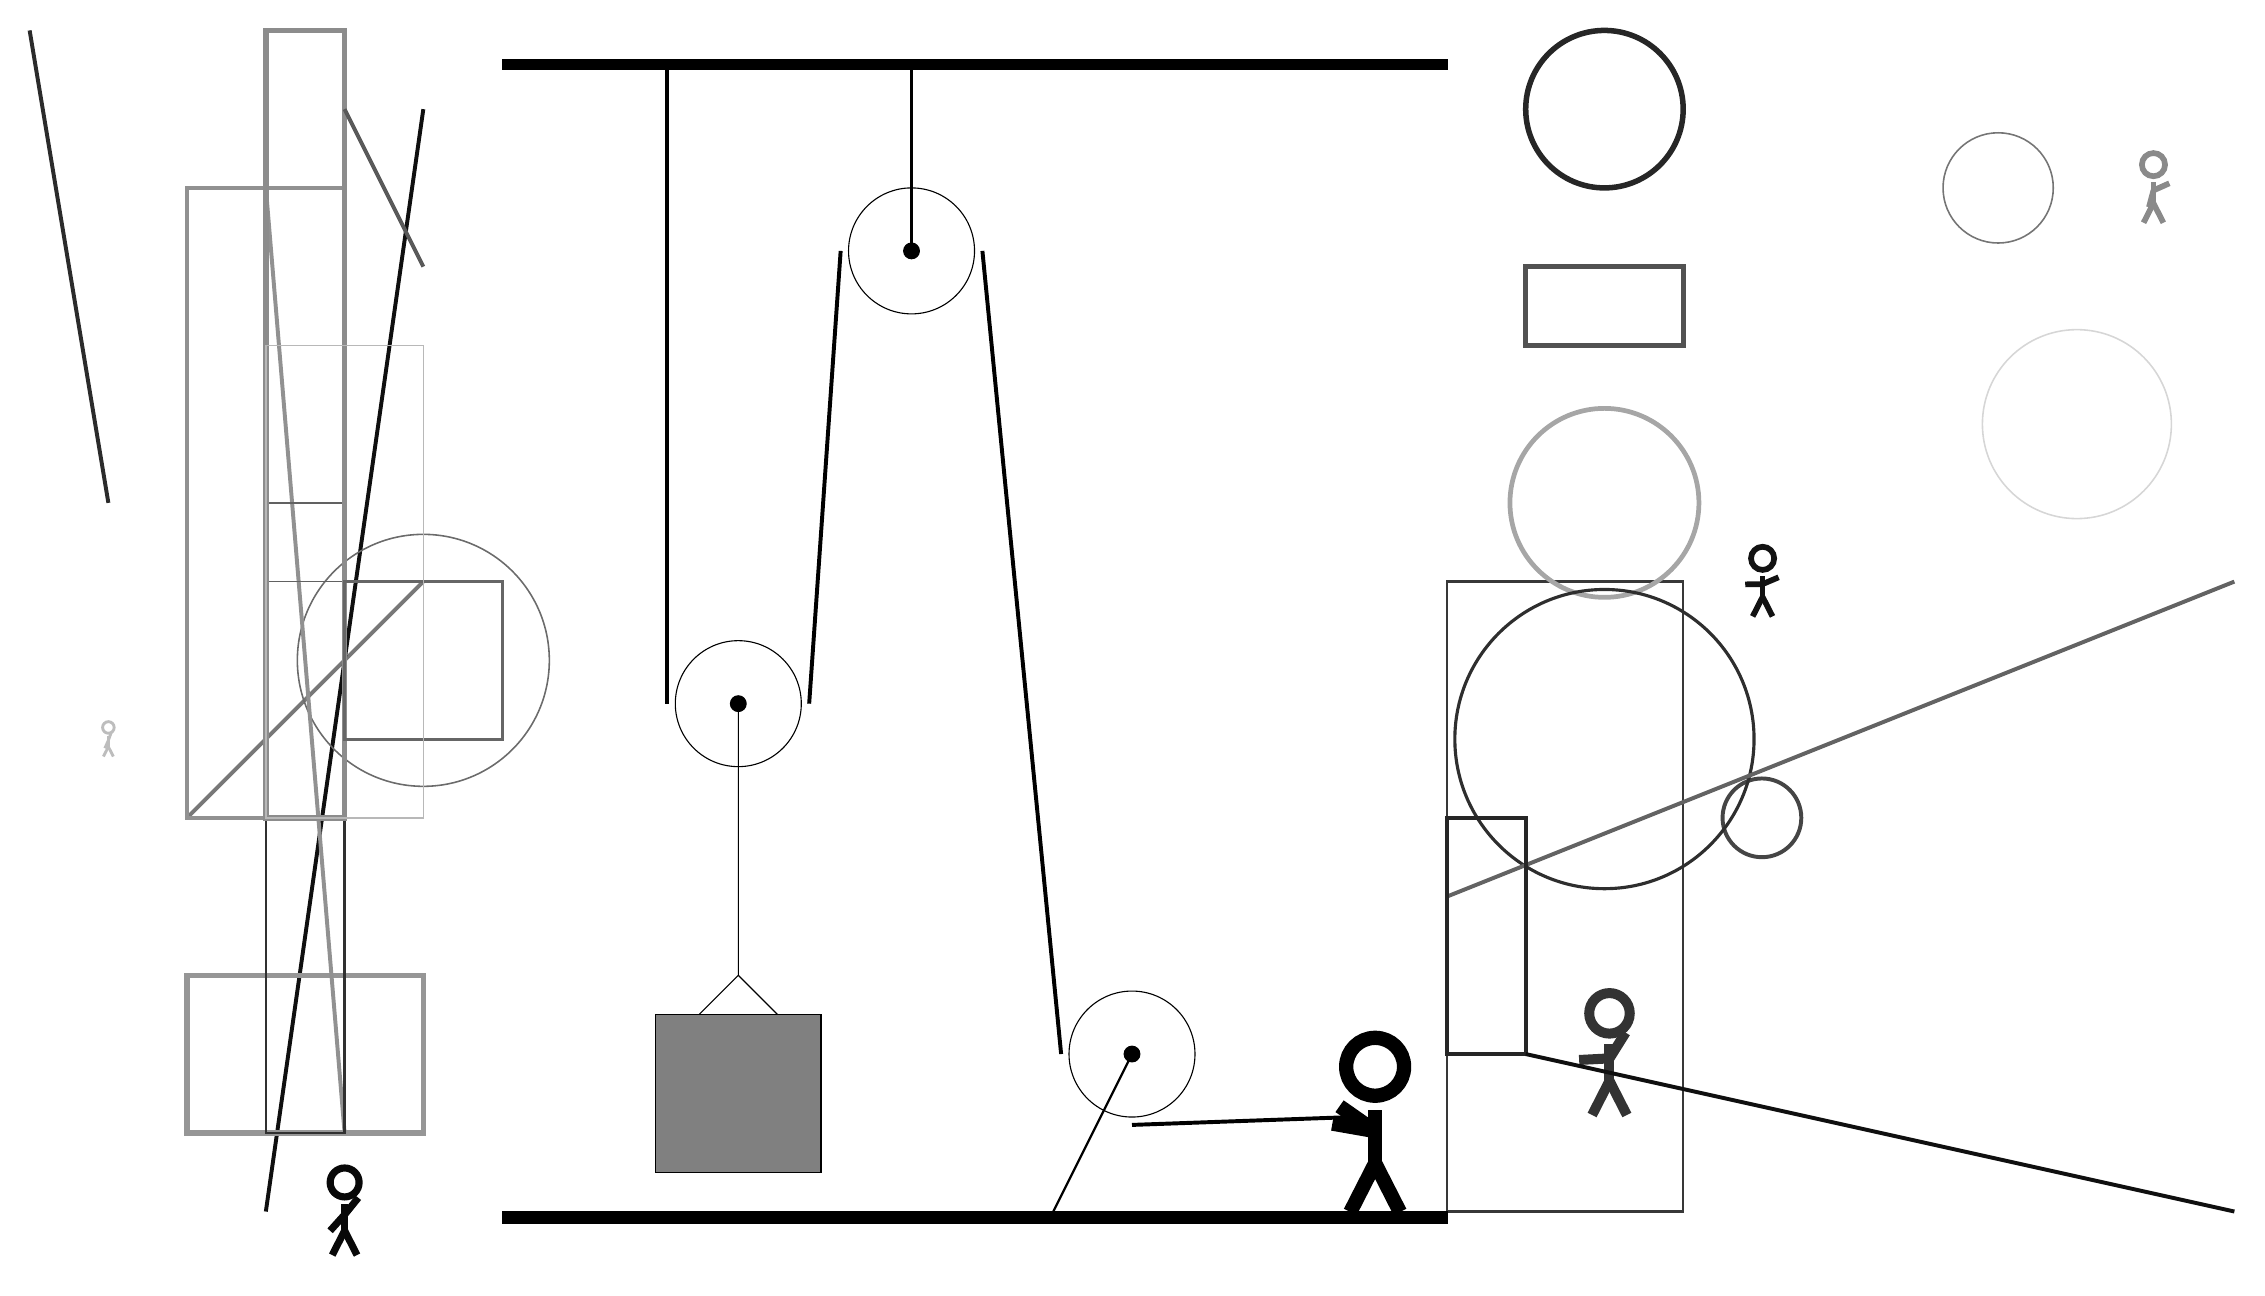
\begin{tikzpicture}
			%%%%% START %%%%%
			
			\draw[fill=black] (-2, 11.5) rectangle (10, 11.625);
			
			\draw (3.2, 9.2) circle (0.8);
			\draw[fill=black] (3.2, 9.2) circle (0.1);
			\draw[thick] (3.2, 9.2) -- (3.2, 11.5);
			
			\draw (6, -1) circle (0.8);
			\draw[fill=black] (6, -1) circle (0.1);
			\draw[thick] (6, -1) -- (5, -3);
			
			\draw (1, 3.45) circle (0.8);
			\draw[fill=black] (1, 3.45) circle (0.1);
			
			\draw (1, 3.45) -- (1, 0.0) -- (0.5, -0.5);
			\draw (1, 0.0) -- (1.5, -0.5);
			\draw[fill=black!50] (-0.05, -0.5) rectangle (2.05, -2.5);
			
			\draw[line width=0.5mm] (0.1, 11.5) -- (0.1, 3.45);
			\centerarc[line width=0.5mm](1, 3.45)(180:360:0.9);
			\draw[line width=0.5mm](1.9, 3.45) -- (2.3, 9.2);
			\centerarc[line width=0.5mm](3.2, 9.2)(0:180:0.9);
			\draw[line width=0.5mm](4.1, 9.2) -- (5.1, -1);
			\centerarc[line width=0.5mm](6, -1)(180:270:0.9);
			\draw[line width=0.5mm](6, -1.9) -- (8.8, -1.8);
			
			\node[line width=0.6mm, color=black!26] at (-7, 3) {\Strichmaxerl[2][66][70]};
			
			\draw[line width=0.5mm, color=black!53](-6, 2) -- (-3, 5);
			\draw [line width=0.5mm, color=black!73](14, 2) circle (0.5);
			\draw [line width=0.2mm, color=black!54](17, 10) circle (0.7);
			\draw[line width=0.3mm, color=black!78] (10, -3) rectangle (13, 5);
			\draw [line width=0.6mm, color=black!35](12, 6) circle (1.2);
			\draw[line width=0.5mm, color=black!94](-3, 11) -- (-5, -3);
			\draw [line width=0.2mm, color=black!58](-3, 4) circle (1.6);
			\draw [line width=0.7mm, color=black!85](12, 11) circle (1.0);
			\draw[line width=0.5mm, color=black!83](-7, 6) -- (-8, 12);
			
			\draw[line width=0.5mm, color=black!43] (-4, 2) rectangle (-6, 10);
			
			\draw[line width=0.7mm, color=black!41] (-3, -2) rectangle (-6, 0);
			\draw [line width=0.4mm, color=black!82](12, 3) circle (1.9);
			
			\draw[line width=0.5mm, color=black!61](10, 1) -- (20, 5);
			\node[line width=0.2mm, color=black!93] at (14, 5) {\Strichmaxerl[4][1][23]};
			\draw [line width=0.2mm, color=black!16](18, 7) circle (1.2);
			
			\draw[line width=0.5mm, color=black!43](-4, -2) -- (-5, 10);
			\node[line width=0.4mm, color=black!46] at (19, 10) {\Strichmaxerl[4][75][24]};
			\draw[line width=0.3mm, color=black!35] (-4, -1) rectangle (-4, 6);
			\node[line width=0.2mm, color=black!97] at (-4, -3) {\Strichmaxerl[5][48][51]};
			\node[line width=0.7mm, color=black!80] at (12, -1) {\Strichmaxerl[7][3][58]};
			\draw[line width=0.3mm, color=black!81] (-4, -2) rectangle (-5, 6);
			\draw[line width=0.2mm, color=black!62] (-4, 5) rectangle (-5, 6);
			\draw[line width=0.7mm, color=black!45] (-4, 2) rectangle (-5, 12);
			\draw[line width=0.5mm, color=black!85] (11, -1) rectangle (10, 2);
			
			\draw[line width=0.6mm, color=black!68] (11, 8) rectangle (13, 9);
			\draw[line width=0.5mm, color=black!65](-3, 9) -- (-4, 11);
			\draw[line width=0.5mm, color=black!94](11, -1) -- (20, -3);
			\draw[line width=0.4mm, color=black!60] (-4, 3) rectangle (-2, 5);
			
			\draw[line width=0.2mm, color=black!28] (-3, 2) rectangle (-5, 8);
			
			\node at (9, -1.9) {\Strichmaxerl[10][-35][170]};
			
			\draw[fill=black] (-2, -3) rectangle (10, -3.15);
			
			%%%%% END %%%%%
		\end{tikzpicture}
	\end{figure}	
\end{document}